\documentclass{article}

\usepackage{ragged2e}
\usepackage{graphicx}
\usepackage{amsmath}
\usepackage{siunitx}
\usepackage{hyperref}

% This stuff is for figures, don't copy-paste
\usepackage{float}
%\DeclareGraphicsExtensions{.png, .pdf}
\DeclareGraphicsExtensions{.pdf, .png}

\renewcommand{\c}[1]{\texttt{#1}}

\begin{document}

%\begin{flushright}
    \noindent
    Rodrigo Becerril Ferreyra\\
    ID 017584071\\
    E E 381 Section 12\\
    Lab 1\\
    Date: 18 September 2020
%\end{flushright}

\addcontentsline{toc}{section}{Introduction}
\section*{Introduction} The purpose of this lab is to get
familiarized with Python, Anaconda, and modeling
probabilities computationally.

\section{Problem 1}
\subsection{Question} The purpose of this Problem is to
create a function that takes in a \(1\text{-by-}n\)
probability vector \(p\)
(whose elements \(p_1, p_2, \ldots , p_n\) are chosen such that
\(\sum_{i=1}^n p_i = 1\))
and return a random integer in the interval \([1, n]\)
according to the probability vector.
This function is named \c{nSidedDie(p)}.

\subsection{Results} The function was tested \num{10000}
times with the probability vector\\
\(p = [0.10, 0.15, 0.20, 0.05, 0.30, 0.10, 0.10]\)
in order to check that the function worked correctly.
The expected result is a high number of \num{5}s and
\num{3}s with a low number of \num{1}s, \num{6}s, and \num{7}s.
In short, the ratio of the number of \(i\)s to the total
number of values (\num{10000}) should be approximate to the \(i\)-th
index in the probability vector. Figure 1 is the image of
the graph generated by the set of values.
Note that this simulation took about \SI{0.13}{s}.

\begin{figure}[H]
    \centering
    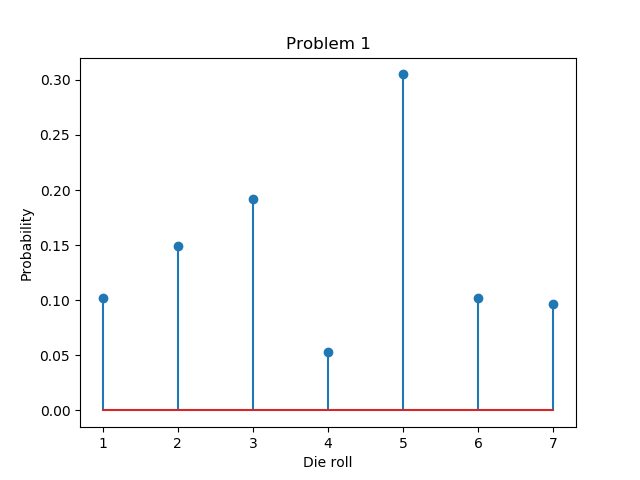
\includegraphics[height=162pt]{Images/Problem1}
    \caption{The Probability Mass Function graph.}
    \label{prob1}
\end{figure}

\section{Problem 2}
\subsection{Question} The purpose of this Problem is to
create an experiment in which two fair, six-sided dice
are rolled until the values on the top faces add up to
\num{7} (which is defined to be a ``success'').
The number of rolls that were taken in order to reach a
success is then recorded, and the experiment is repeated
\num{100000} times. The values of the successes are then
plotted against the amount of times that they occurred out of
\num{100000} on a stem plot.

\subsection{Results} Figure 2 is the image of the stem plot
generated. It is easy to see that the majority of times,
a success was reached on the first roll. The next points
decline exponentially until hitting about one occurrence
at the end. Note that this simulation took about \SI{1.88}{s}.

\begin{figure}[H]
    \centering
    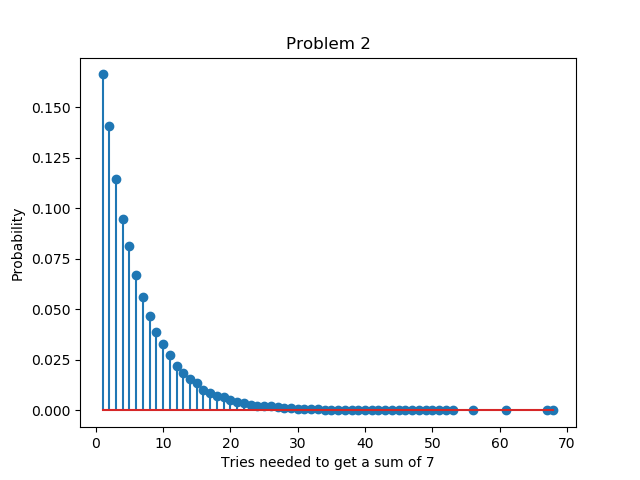
\includegraphics[height=162pt]{Images/Problem2}
    \caption{Stem plot of rolls.}
    \label{prob2}
\end{figure}

\section{Problem 3}
\subsection{Question} The purpose of this Problem is to devise
and carry out an experiment that calculates the experimental
probability of flipping 100 fair (two-sided) coins and having
exactly \num{50} of them land on heads and \num{50} of them
land on tails.

\pagebreak

\subsection{Results} To calculate this probability
to a certain degree of precision,
it was necessary to perform the experiment explained in Section
3.1 \num{100000} times. Table 1 describes the probability
found in doing so. Note that this simulation took about
\SI{15}{\second}.

\begin{table}[H]
    \centering\begin{tabular}{| r | l |}
        \hline
        Prob. of 50 heads in tossing 100 fair coins & \\ \hline
        \textbf{Ans.} & \(p \approx \num{8.000e-2} \pm \num{2e-3}\) \\ \hline
    \end{tabular}
    \caption{A table containing the probability.}
    \label{prob3}
\end{table}

\section{Problem 4}
\subsection{Question} The purpose of this problem is to
apply probability to real-life applications, such as
security. The scenario is as follows: a hacker makes a list
of \(m\) random lowercase four-letter words (repetitions
allowed) to test on a password system. What is the probability
that the hacker gets into the password system (in other words,
the probability that the correct password matches one or
more of the hacker's attempted passwords)? It is assumed
that only four-letter words with lowercase letters are
allowed, for simplicity.

This Problem is split into three parts:
\begin{enumerate}
    \item Let the hacker create a list of \(m\) words.
    \item Let the hacker create a list of \(km\) words.
    \item Find the length of the hacker's list in which the
    hacker has a \num{50}\% chance of hacking into the system.
\end{enumerate}

For this problem, the values of \(m = \num{80000}\) and \(k = 7\)
were given.

\subsection{Results} To achieve a certain degree of precision
in the calculation of the probability, each test was
performed \num{1000} times. Part 1's list was
\(m = \num{80000}\) words long, and Part 2's list was
\(km = \num{560000}\) words long. Figure 3
shows the output of these two experiments. Note that
Test 1 took \SI{200.88}{s} and Test 2 took \SI{1430.49}{s}.

\begin{figure}[H]
    \centering
    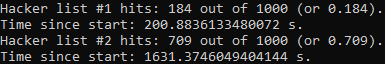
\includegraphics{Images/hacker}
    \caption{Output for Problem 4 Tests 1 and 2.}
    \label{prob4:test12}
\end{figure}

The third part of this Problem is to find the value of \(m\)
such that a list of \(m\) words gives the hacker a 50\% chance
of succeeding. I estimated the value of \(m\) in the following
way.

\begin{figure}[h]
    \centering
    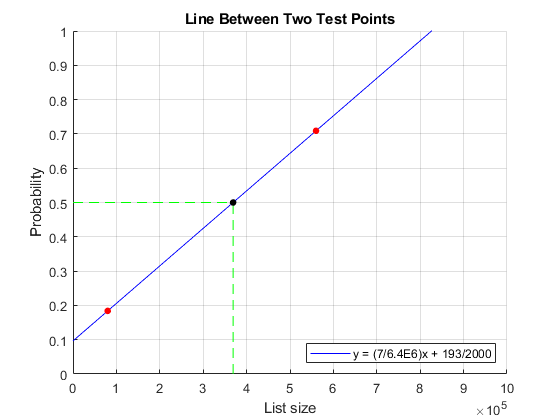
\includegraphics[height=162pt]{Images/LineBetweenTwoTestPoints.png}
    \caption{Estimation of \(m\).}
    \label{LineBetweenTwoTestPoints}
\end{figure}

First, I plotted the two results that I achieved in
Part 1 and Part 2 (the ordered pairs
\((\num{80000}, 0.184)\) and \((\num{560000}, 0.709)\)),
and drew a line between them:\begin{equation*}
    y = \frac{7}{\num{6.4E6}}x + \frac{193}{2000}
\end{equation*} Then, I solved the equation for \(x\) given
that \(y = 0.5\), to see how long the list of passwords needs
to be to obtain the probability of \num{0.5}; the answer
comes out to be \(x = \num{2582400/7} \approx \num{368914}\).
In doing this, I assumed that the probability can be
described using a linear function.

Figure 5 is the output of the experiment using a hacker
list of \num{368914} words. The probability is \num{0.553},
which is close to the goal of \num{0.500}.
Note that this simulation took
about \SI{925.84}{s}.

\begin{figure}[H]
    \centering
    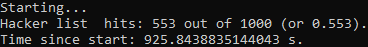
\includegraphics{Images/hacker3}
    \caption{Output for Problem 4 Test 3}
    \label{prob4:test3}
\end{figure}

Table 2 is a compilation of all aforementioned results.

\begin{table}[H]
    \centering\begin{tabular}{| r | l |}
        \hline
        Prob. at least 1 word in \(m\)-sized list matches the password: & \(p = 0.184\) \\ \hline
        Prob. at least 1 word in\(km\)-sized list matches the password: & \(p = 0.709\) \\ \hline
        Approx. num. of words in list needed to obtain  \(p = 0.500\) & \(m = \num{368914}\) \\ \hline
    \end{tabular}
    \caption{Table of results for Problem 4.}
    \label{prob4:table}
\end{table}

\end{document}
